\documentclass[10pt, conference]{IEEEtran}

\usepackage[english]{babel}
\usepackage{amsmath}
\usepackage{amssymb}
\usepackage{booktabs}
\usepackage{enumitem}
\usepackage{algorithm}
\usepackage{algorithmic}
\usepackage{graphicx}
\usepackage{hyperref}
\usepackage{tikz}
\usetikzlibrary{positioning, arrows.meta, shapes.geometric, calc, fit, backgrounds}

% Custom macro to safely load images or fallback to a placeholder if the file is missing
\newcommand{\safeimage}[2][]{%
    \IfFileExists{#2}{%
        \includegraphics[#1]{#2}%
    }{%
        \framebox{\parbox{0.45\textwidth}{\centering
        \vspace{2cm}
        \textbf{Image Placeholder} \\
        \small\textit{\detokenize{#2}}
        \vspace{2cm}}}%
    }%
}

\begin{document}

\title{AEGIS: A Byzantine-Resilient Federated Learning Protocol for Highly Non-IID Environments}

\author{
\IEEEauthorblockN{Anonymous Author 1}
\IEEEauthorblockA{\textit{Anonymous Department 1} \\
\textit{Anonymous Institution 1}\\
City, Country \\
author1@example.com}
\and
\IEEEauthorblockN{Anonymous Author 2}
\IEEEauthorblockA{\textit{Anonymous Department 2} \\
\textit{Anonymous Institution 2}\\
City, Country \\
author2@example.com}
}

\maketitle

\begin{abstract}
Federated Learning (FL) is vulnerable to Byzantine attacks, where compromised clients submit poisoned updates to degrade the global model. Existing robust aggregators force a harsh tradeoff: distance-based methods incur a prohibitive $\mathcal{O}(k^2d)$ computational bottleneck and mistakenly penalize honest statistical drift, while highly efficient $\mathcal{O}(kd)$ coordinate-wise median filters remain fundamentally blind to directional poisoning. The objective of this work is to bridge this gap, delivering dual-metric robustness without sacrificing linear scalability. To this end, we introduce \textit{Aegis}, an aggregation protocol designed for environments with high data skew. Operating with an asymptotic complexity of $\mathcal{O}(kd)$, Aegis replaces standard distance-based filters with a two-pass dual-metric anomaly detection system, utilizing adaptive Median Absolute Deviation (MAD) thresholding and cross-round reputation tracking. We evaluate Aegis on CIFAR-10 under a 30\% Byzantine threat model. Under a 30\% Byzantine threat, Aegis holds accuracy within 10\% of the clean baseline across Sign-Flipping, Label-Flipping, and Volume Spam — without sacrificing linear scalability. However, we also explicitly document the breaking points of statistical filtering: while the two-pass architecture improves resilience against Inner Product Manipulation (IPM), variance-envelope attacks (such as ALIE) and majority-hijacking Sybil attacks can overwhelm median-based anchors entirely.
\end{abstract}

\begin{IEEEkeywords}
Federated Learning, Byzantine Resilience, Model Poisoning, Non-IID Data, Robust Aggregation, Sybil Attacks, Volume Spam, ALIE Attack, Inner-Product Manipulation, Gradient Clipping, Cosine Similarity, Median Absolute Deviation.
\end{IEEEkeywords}

\section{Introduction}
Federated Learning (FL) enables edge devices to collaboratively train a shared global model without exchanging raw, privacy-sensitive data. However, this decentralized architecture introduces a critical attack vector: Byzantine clients. Whether compromised by attackers or suffering from hardware faults, these nodes can transmit poisoned model updates to degrade accuracy, insert backdoors, or prevent convergence \cite{blanchard2017}.

Securing FL is complicated by the statistical heterogeneity of real-world edge data. In highly Non-IID environments, legitimate clients often produce weight updates that diverge from the global average simply due to local data skew. Standard robust aggregators penalize this natural diversity — discarding legitimate updates from honest clients whose local distributions simply reflect real-world data skew. On top of that, distance-based methods like Krum scale quadratically $\mathcal{O}(k^2 d)$ with the number of participating clients, posing theoretical bottlenecks for massively distributed set of clients.

We propose \textbf{Aegis} to address these limitations. The protocol separates adversarial anomalies from natural Non-IID variance using a two-pass median decontamination process, adaptive credit scoring, and historical reputation tracking. The reputation system provides marginal improvement under colluding (non-omniscient) ALIE and contributes to credit scoring under conventional attacks where it accumulates meaningful signal. Rather than relying on a single spatial metric, Aegis evaluates Euclidean distance and Cosine similarity simultaneously. It applies MAD-based adaptive thresholds to these metrics, automatically adjusting to the client's update variance each round. In our evaluation, we demonstrate robust defense against conventional attacks, compare empirical execution dynamics against baseline aggregators, and explicitly document the limits of statistical filtering against advanced optimization attacks like ALIE and Sybil.

\section{Related Work}
Byzantine resilience in FL has been approached from several directions, each with distinct trade-offs in computational cost, threat coverage, or privacy assumptions.

\textbf{Distance-Based Aggregators:} Krum and Multi-Krum \cite{blanchard2017} select updates using pairwise distances. They provide provable resilience but theoretically require $\mathcal{O}(k^2 d)$ computations. Importantly, distance selection frequently fails against optimization-based attacks like ALIE \cite{baruch2019}. Bulyan \cite{elmhamdi2018} attempts to fix Krum's vulnerabilities via a two-phase meta-aggregation, but the $\mathcal{O}(k^3 d)$ cost is prohibitive.

\textbf{Statistical and Spectral Methods:} Trimmed Mean and Coordinate-wise Median \cite{yin2018} operate efficiently but assume coordinate-wise independence, leaving them vulnerable to Inner Product Manipulation (IPM) attacks \cite{xie2020ipm}. Divide-and-Conquer (DnC) \cite{shejwalkar2021} employs spectral methods to detect correlated perturbations but incurs significant computational overhead. A recent meta-analysis \cite{allouah2025} confirms that optimization-based attacks continue to bypass standard statistical rules.

\textbf{Trust and Hybrid Defenses:} FLTrust \cite{cao2021} and Zeno \cite{xie2019zeno} score updates against a server-side root dataset. This approach violates pure FL privacy norms and struggles in extreme Non-IID settings where the server data may not reflect edge distributions. FLAME \cite{nguyen2022} combines cosine-based clustering and adaptive clipping, serving as a precedent for angular pre-screening, but relies on $\mathcal{O}(k^2 d)$ HDBSCAN clustering. While trust-based defenses like CONTRA \cite{awan2021contra} track accumulated gradient histories and leverage $\mathcal{O}(k^2)$ pairwise cosine similarities to detect colluding Sybils, Aegis targets resilience through robust multi-metric filtering and scalar reputation tracking against an $\mathcal{O}(kd)$ cleansed median, avoiding pairwise computational bottlenecks and without relying on global momentum buffers or external clean datasets.

\section{Threat Model and Environment}

\subsection{System Architecture and Data Heterogeneity}
We consider a cross-device FL architecture with a central parameter server and $n = 30$ clients. To simulate realistic data skew, we use Shard-based partitioning \cite{mcmahan2017}. The dataset is sorted by label, and each client is allocated exactly 4 random data shards, ensuring no single client holds a representative sample of the global distribution.

\subsection{Adversary and Participation Model}
We evaluate Aegis under a \textit{Fixed Adversary with Random Participation} model. The identities of compromised nodes are fixed at the start of training. During each round, a random subset of clients $m \in [15, 25]$ is selected. Consequently, the exact number of participating Byzantine clients follows a Hypergeometric distribution:
\begin{equation}
X \sim \text{Hypergeometric}(N=30, f=9, m)
\end{equation}
where $f=9$ represents a 30\% global Byzantine presence and $m$ is the number of clients sampled per round. In our Sybil evaluations, each physical adversary operates with a multiplicity of 2, generating two distinct synthetic identities to assess the protocol's resilience against identity-spoofing collusion.

\subsection{Attack Hierarchy}
We categorize the evaluated threats into three distinct vectors: vector-level gradient manipulation, metadata/label poisoning, and structural identity attacks.

\begin{enumerate}
    \item \textbf{Gradient-Level Vector Manipulation:}
    \begin{itemize}
        \item \textit{Sign-Flipping:} Byzantine clients negate their local pseudo-gradients ($\Delta_k = -1 \times \Delta_{\text{local}}$) before submission to steer the global model towards divergence.
        \item \textit{Gaussian Noise Injection:} Malicious updates are perturbed with additive white noise ($\sigma=2.0$) to degrade convergence stability and increase the global loss.
        \item \textit{Inner Product Manipulation (IPM) \cite{xie2020ipm}:} Attackers compute the mean gradient $\mu$ of the collective's updates and submit a scaled inverse $(\Delta_k = -\epsilon \mu)$ where $\epsilon=0.5$. This targeted attack is designed to force the global update into a state of gradient ascent.
        \item \textit{A Little Is Enough (ALIE) \cite{baruch2019}:} An omniscient adversary crafts poisoned vectors that lie strictly within the variance envelope of the honest client distributions (quantified by a cumulative distribution threshold $z=1.0$), bypassing statistical filters that rely on crude outlier detection.
    \end{itemize}
    
    \item \textbf{Data and Metadata Poisoning:}
    \begin{itemize}
        \item \textit{Targeted Label-Flipping:} Adversaries perform complement label-flipping ($y_{\text{poisoned}} = (C-1) - y$) to induce specific misclassifications while maintaining high reported confidence.
        \item \textit{Volume Spam:} Attackers artificially inflate their reported sample size $n_k$ to hijack the weighted average in standard aggregators like FedAvg.
    \end{itemize}
    
    \item \textbf{Structural and Identity Attacks:}
    \begin{itemize}
        \item \textit{Sybil \& Collusion:} Multiple adversarial identities coordinate their updates to overwhelm the median anchor. In our evaluation, each physical adversary operates with a multiplicity of 2 to simulate a majority-hijacking scenario.
    \end{itemize}
\end{enumerate}

\section{The AEGIS Protocol: Mechanics \& Architecture}

% =====================================================================
% AEGIS Architecture Diagram — IEEE Two-Column Compatible
% =====================================================================
% Preamble requirements:
%   \usepackage{tikz}
%   \usetikzlibrary{shapes.geometric, arrows.meta, positioning, 
%                    calc, fit, backgrounds}
%
% Uses figure* for full-width spanning both IEEE columns.
% Tested with IEEEtran class at \textwidth ~ 7.0in (17.78cm).
% =====================================================================

\begin{figure*}[!t]
\centering
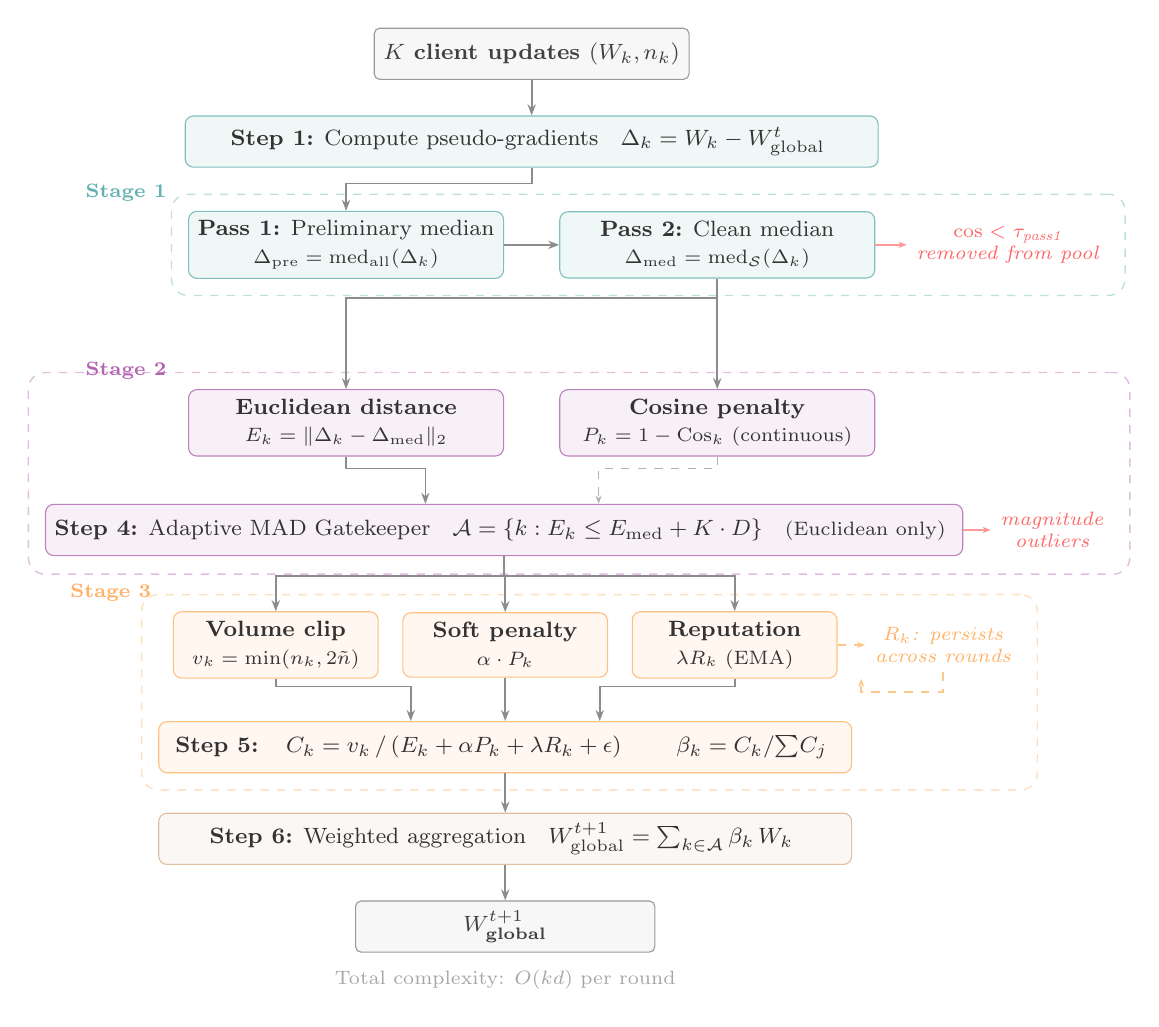
\begin{tikzpicture}[
    node distance=0.5cm and 0.6cm,
    % --- Node Styles ---
    iobox/.style={
        rectangle, rounded corners=2pt, draw=black!40, fill=gray!6,
        minimum width=3.8cm, minimum height=0.65cm,
        font=\footnotesize\bfseries, text=black!75, align=center
    },
    procbox/.style={
        rectangle, rounded corners=3pt, draw=#1!50, fill=#1!6,
        minimum width=4.0cm, minimum height=0.65cm,
        font=\footnotesize, text=black!80, align=center
    },
    procbox/.default={blue},
    wideprocbox/.style={
        rectangle, rounded corners=3pt, draw=#1!50, fill=#1!6,
        minimum width=8.8cm, minimum height=0.65cm,
        font=\footnotesize, text=black!80, align=center
    },
    wideprocbox/.default={blue},
    smallbox/.style={
        rectangle, rounded corners=3pt, draw=orange!50, fill=orange!6,
        minimum width=2.6cm, minimum height=0.65cm,
        font=\footnotesize, text=black!80, align=center
    },
    rejectlbl/.style={
        font=\scriptsize\itshape, text=red!60, align=center
    },
    feedlbl/.style={
        font=\scriptsize\itshape, text=orange!60, align=center
    },
    stagelbl/.style={
        font=\scriptsize\bfseries, text=#1!60
    },
    stagelbl/.default={blue},
    % --- Arrow Styles ---
    ar/.style={-{Stealth[length=4pt]}, draw=black!45, semithick},
    dar/.style={-{Stealth[length=3pt]}, dashed, draw=black!30},
    rar/.style={-{Stealth[length=3pt]}, draw=red!40, semithick},
    far/.style={-{Stealth[length=3pt]}, dashed, draw=orange!45, semithick},
    % --- Stage Frame ---
    sframe/.style={
        rectangle, rounded corners=6pt, draw=#1!25,
        dashed, line width=0.5pt, inner sep=6pt
    },
    sframe/.default={blue},
]

% ==================== STEP 2: TWO-PASS (placed first as layout anchor) ====================
\node[procbox={teal}] (pass1) {
    \textbf{Pass 1:} Preliminary median\\[0.5pt]
    {\scriptsize $\Delta_{\text{pre}} = \text{med}_{\text{all}}(\Delta_k)$}
};
\node[procbox={teal}, right=0.7cm of pass1] (pass2) {
    \textbf{Pass 2:} Clean median\\[0.5pt]
    {\scriptsize $\Delta_{\text{med}} = \text{med}_{\mathcal{S}}(\Delta_k)$}
};
\node[rejectlbl, right=0.4cm of pass2] (rej1) {
    $\cos < \tau_{\text{pass1}}$\\removed from pool
};

% ==================== INPUT & STEP 1 (centered above pass1-pass2 midpoint) ====================
\node[wideprocbox={teal}, above=0.55cm of $(pass1.north)!0.5!(pass2.north)$] (step1) {
    \textbf{Step 1:} Compute pseudo-gradients \;
    $\Delta_k = W_k - W^t_{\text{global}}$
};
\node[iobox, above=0.45cm of step1] (input) {$K$ client updates $(W_k, n_k)$};

% ==================== STEP 3: DUAL SCORING ====================
\node[procbox={violet}, below=1.4cm of pass1] (euclid) {
    \textbf{Euclidean distance}\\[0.5pt]
    {\scriptsize $E_k = \|\Delta_k - \Delta_{\text{med}}\|_2$}
};
\node[procbox={violet}, right=0.7cm of euclid] (cossim) {
    \textbf{Cosine penalty}\\[0.5pt]
    {\scriptsize $P_k = 1 - \text{Cos}_k$ (continuous)}
};

% ==================== STEP 4: GATEKEEPER ====================
\node[wideprocbox={violet}, below=0.6cm of euclid.south east] (gate) {
    \textbf{Step 4:} Adaptive MAD Gatekeeper \;
    $\mathcal{A} = \{k : E_k \leq E_{\text{med}} + K \cdot D\}$
    \; {\scriptsize (Euclidean only)}
};
\node[rejectlbl, right=0.35cm of gate] (rej2) {
    magnitude\\outliers
};

% ==================== STEP 5: CREDIT SCORING ====================
\node[smallbox, below=0.7cm of gate, xshift=-2.9cm] (vol) {
    \textbf{Volume clip}\\[0.5pt]
    {\scriptsize $v_k = \min(n_k, 2\tilde{n})$}
};
\node[smallbox, right=0.3cm of vol] (pen) {
    \textbf{Soft penalty}\\[0.5pt]
    {\scriptsize $\alpha \cdot P_k$}
};
\node[smallbox, right=0.3cm of pen] (rep) {
    \textbf{Reputation}\\[0.5pt]
    {\scriptsize $\lambda R_k$ (EMA)}
};

\node[wideprocbox={orange}, below=0.55cm of pen] (credit) {
    \textbf{Step 5:} \;
    $C_k = v_k \,/\, (E_k + \alpha P_k + \lambda R_k + \epsilon)$
    \qquad $\beta_k = C_k / {\textstyle\sum} C_j$
};

% Feedback annotation
\node[feedlbl, right=0.35cm of rep] (fblbl) {
    $R_k$: persists\\across rounds
};

% ==================== STEP 6: AGGREGATION ====================
\node[wideprocbox={brown}, below=0.5cm of credit] (agg) {
    \textbf{Step 6:} Weighted aggregation \;
    $W^{t+1}_{\text{global}} = \sum_{k \in \mathcal{A}} \beta_k \, W_k$
};

% ==================== OUTPUT ====================
\node[iobox, below=0.45cm of agg] (output) {$W^{t+1}_{\text{global}}$};

% ==================== ARROWS ====================
% Main vertical flow
\draw[ar] (input) -- (step1);
\draw[ar] (step1.south) -- ++(0,-0.2) -| (pass1.north);
\draw[ar] (pass1) -- (pass2);

% Pass 1 reject
\draw[rar] (pass2.east) -- (rej1.west);

% Pass 2 to dual scoring
\draw[ar] (pass2.south) -- ++(0,-0.25) -| (euclid.north);
\draw[ar] (pass2.south) -- ++(0,-0.25) -| (cossim.north);

% Dual scoring to gate
\draw[ar] (euclid.south) -- ++(0,-0.15) -| ([xshift=-1cm]gate.north);
% Cosine feeds THROUGH gate to credit (dashed = bypasses hard gate)
\draw[dar] (cossim.south) -- ++(0,-0.15) -| ([xshift=1.2cm]gate.north);

% Gate reject
\draw[rar] (gate.east) -- (rej2.west);

% Gate to scoring inputs
\draw[ar] (gate.south) -- ++(0,-0.25) -| (vol.north);
\draw[ar] (gate.south) -- ++(0,-0.25) -| (pen.north);
\draw[ar] (gate.south) -- ++(0,-0.25) -| (rep.north);

% Scoring inputs to credit formula
\draw[ar] (vol.south) -- ++(0,-0.1) -| ([xshift=-1.2cm]credit.north);
\draw[ar] (pen.south) -- (credit.north);
\draw[ar] (rep.south) -- ++(0,-0.1) -| ([xshift=1.2cm]credit.north);

% Reputation feedback loop
\draw[far] (rep.east) -- (fblbl.west);
\draw[far] (fblbl.south) |- ++(0,-0.25) -| ([xshift=0.3cm]rep.south east);

% Credit to aggregation
\draw[ar] (credit) -- (agg);

% Aggregation to output
\draw[ar] (agg) -- (output);

% ==================== STAGE LABELS ====================
\node[stagelbl={teal}, left=0.15cm of pass1.north west, anchor=south east] {
    Stage 1
};
\node[stagelbl={violet}, left=0.15cm of euclid.north west, anchor=south east] {
    Stage 2
};
\node[stagelbl={orange}, left=0.15cm of vol.north west, anchor=south east] {
    Stage 3
};

% ==================== STAGE FRAMES ====================
\begin{scope}[on background layer]
    \node[sframe={teal}, fit=(pass1)(pass2)(rej1)] {};
    \node[sframe={violet}, fit=(euclid)(cossim)(gate)(rej2)] {};
    \node[sframe={orange}, fit=(vol)(rep)(credit)(fblbl)] {};
\end{scope}

% ==================== COMPLEXITY NOTE ====================
\node[font=\scriptsize, text=black!35, below=0.1cm of output] {
    Total complexity: $O(kd)$ per round
};

\end{tikzpicture}

\caption{AEGIS aggregation pipeline. Stage~1 decontaminates the 
coordinate-wise median via two-pass cosine pre-screening 
($\tau_{\text{pass1}} = -0.3$). Stage~2 applies an adaptive 
MAD-based Euclidean filter as the sole hard gate. The cosine 
penalty $P_k$ bypasses the hard gate (dashed arrow) and enters 
the soft credit score in Stage~3, where it combines with volume 
bounds and cross-round reputation $R_k$ to produce normalized 
aggregation weights $\beta_k$. No hard directional threshold is 
applied; directional suppression is entirely continuous via 
$\alpha P_k$ in the credit score denominator.}
\label{fig:aegis-arch}
\end{figure*}
\begin{algorithm}[htbp]
\caption{AEGIS: Two-Pass Byzantine-Resilient Aggregation with Soft Directional Penalty}
\label{alg:aegis}
\begin{algorithmic}[1]

\REQUIRE Updates $\{(W_k, n_k)\}_{k=1}^{K}$, global model $W^t_{\text{global}}$, round $t$, reputation state $\{R_k\}$
\ENSURE Aggregated model $W^{t+1}_{\text{global}}$

\STATE \textbf{// Step 1: Compute Pseudo-Gradients}
\FOR{each client $k$}
    \STATE $\Delta_k \leftarrow W_k - W^t_{\text{global}}$
\ENDFOR

\STATE

\STATE \textbf{// Step 2: Two-Pass Robust Center (Median Decontamination)}
\STATE $\Delta_{\text{pre}} \leftarrow \text{median}_k(\Delta_k)$ \hfill $\blacktriangleright$ \textit{Pass 1: Preliminary median}
\FOR{each client $k$}
    \STATE $\text{cos}^{\text{pre}}_k \leftarrow \frac{\Delta_k \cdot \Delta_{\text{pre}}}{\|\Delta_k\|_2 \|\Delta_{\text{pre}}\|_2}$
\ENDFOR
\STATE $\mathcal{S} \leftarrow \{k : \text{cos}^{\text{pre}}_k \geq \tau_{\text{pass1}}\}$ \hfill $\blacktriangleright$ \textit{Screen adversarial directions}
\STATE $\Delta_{\text{med}} \leftarrow \text{median}_{k \in \mathcal{S}}(\Delta_k)$ \hfill $\blacktriangleright$ \textit{Pass 2: Debiased clean median}

\STATE

\STATE \textbf{// Step 3: Dual Anomaly Scoring (all clients re-scored)}
\FOR{each client $k$}
    \STATE $E_k \leftarrow \|\Delta_k - \Delta_{\text{med}}\|_2$ \hfill $\blacktriangleright$ \textit{Euclidean distance}
    \STATE $\text{Cos}_k \leftarrow \frac{\Delta_k \cdot \Delta_{\text{med}}}{\|\Delta_k\|_2 \|\Delta_{\text{med}}\|_2}$ \hfill $\blacktriangleright$ \textit{Cosine similarity}
    \STATE $P_k \leftarrow 1.0 - \text{Cos}_k$ \hfill $\blacktriangleright$ \textit{Cosine penalty (continuous)}
\ENDFOR

\STATE

\STATE \textbf{// Step 4: Adaptive MAD Gatekeeper (Euclidean only)}
\STATE $E_{\text{med}} \leftarrow \text{median}(E_k)$; \quad $D \leftarrow \text{median}(|E_k - E_{\text{med}}|)$
\STATE $K_{\text{phase}} \leftarrow K_{\max} - (K_{\max} - K_{\min}) \cdot \min\!\left(\frac{t}{t_{\text{warmup}}},\, 1\right)$
\STATE $CV \leftarrow D \;/\; E_{\text{med}}$
\STATE $K \leftarrow \max\!\big(K_{\text{floor}},\; K_{\text{phase}} \cdot (1 + \eta \cdot CV)\big)$
\STATE $T \leftarrow E_{\text{med}} + K \cdot D$
\STATE $\mathcal{A} \leftarrow \{k : E_k \leq T\}$ \hfill $\blacktriangleright$ \textit{Magnitude gate}

\STATE

\STATE \textbf{// Step 5: Volume Bounding, Reputation \& Soft Credit Scoring}
\FOR{each $k \in \mathcal{A}$}
    \STATE $v_k \leftarrow \min(n_k,\; 2.0 \times \text{median}_{j \in \mathcal{A}}(n_j))$ \hfill $\blacktriangleright$ \textit{Volume clip}
    \STATE $R_k \leftarrow \gamma \cdot R_k + (1 - \gamma) \cdot P_k$ \hfill $\blacktriangleright$ \textit{Reputation update (EMA)}
    \STATE $C_k \leftarrow \dfrac{v_k}{E_k + \alpha \cdot P_k + \lambda \cdot R_k}$ \hfill $\blacktriangleright$ \textit{Soft directional suppression}
\ENDFOR
\STATE $\beta_k \leftarrow C_k \;/\; \sum_{j \in \mathcal{A}} C_j$ \hfill $\blacktriangleright$ \textit{Normalized weights}

\STATE

\STATE \textbf{// Step 6: Aggregation}
\STATE $W^{t+1}_{\text{global}} \leftarrow \sum_{k \in \mathcal{A}} \beta_k \cdot W_k$

\RETURN $W^{t+1}_{\text{global}}$

\end{algorithmic}
\end{algorithm}

Aegis executes a 6-step pipeline per round (summarized in Algorithm \ref{alg:aegis} and Figure \ref{fig:aegis-arch}). By utilizing Introselect for median computations and avoiding pairwise distance matrices, Aegis maintains an asymptotic time complexity of $\mathcal{O}(kd)$.

\subsection{Step 1: Distribution \& Local Training}
The server broadcasts $W_{global}^t$. Client $k$ trains locally and returns its updated weights $W_k$ and claimed sample size $n_k$. We compute the local pseudo-gradient: $\Delta_k = W_k - W_{global}^t$.

\subsection{Step 2: Two-Pass Median Decontamination}
Optimization attacks like IPM are specifically designed to drag the standard coordinate-wise median off-center. Once this reference point is compromised, the aggregator begins generating false positives — rejecting legitimate clients whose updates reflect natural data skew rather than adversarial intent. We address this by computing the robust center in two passes, decoupling the reference point from potentially compromised updates.
\begin{enumerate}
    \item \textbf{Pass 1 (Pre-screen):} Compute a preliminary median $\Delta_{pre} = \text{median}_{all}(\Delta_k)$. Compute cosine similarities against $\Delta_{pre}$ and provisionally remove clients where $\cos < \tau_{\text{pass1}}$ (where $\tau_{\text{pass1}} = -0.3$).
    \item \textbf{Pass 2 (Clean Anchor):} Recompute the final robust center solely from the surviving clients: $\Delta_{median} = \text{median}_{clean}(\Delta_k)$.
\end{enumerate}

\subsection{Step 3: Dual Anomaly Scoring}
Every client is evaluated against $\Delta_{median}$. 
First, Euclidean Distance measures the magnitude of the deviation between the client’s update $\Delta_{k}$ and the robust median $\Delta_{\text{median}}$ to detect additive noise:
\begin{equation}
E_k = ||\Delta_k - \Delta_{median}||_2
\end{equation}
Second, Cosine Similarity measures direction to detect Sign and Label-Flipping:
\begin{equation}
Cos_k = \frac{\Delta_k \cdot \Delta_{median}}{||\Delta_k||_2 ||\Delta_{median}||_2} \quad \text{and} \quad P_k = 1.0 - Cos_k
\end{equation}

\subsection{Step 4: Adaptive Thresholding \& Gatekeeper Logic}
Aegis self-calibrates its rejection threshold using Median Absolute Deviation (MAD). Base metrics are: $E_{median} = \text{median}(E_k)$ and $D = \text{median}(|E_k - E_{median}|)$.
An adaptive multiplier ($K$) decays over a warmup period, modulated by the swarm variance ($CV = D / E_{median}$):
\begin{equation}
K_{phase} = K_{max} - (K_{max} - K_{min}) \times \left(\frac{t}{\text{warmup\_rounds}}\right)
\end{equation}
\begin{equation}
K = \max\left(K_{safe\_floor}, K_{phase} \times (1 + \text{Var\_Sensitivity} \times CV)\right)
\end{equation}
The rejection threshold is $T = E_{median} + K \cdot D$. Updates are discarded solely based on magnitude if $E_k > T$.

\subsection{Step 5: Cross-Round Reputation Tracking \& Credit Scoring}
To penalize persistent stealth attackers, the server maintains an exponential moving average (EMA) reputation penalty $R_k$ for each client. This update is applied strictly to approved clients; rejected nodes retain their prior reputation state to prevent adversarial noise from polluting the historical record.
\begin{equation}
R_k^{t+1} = \gamma R_k^t + (1 - \gamma) P_k^t
\end{equation}
To prevent Volume Spam, claimed sizes are clipped relative to the median of the current round's approved clients. By calculating the bounding median over a decontaminated pool, we ensure a minority of high-volume spammers cannot skew the aggregation bounds:
\begin{equation}
v_k = \min(n_k, 2.0 \times \text{median}(n_{approved}))
\end{equation}
The final credit score integrates the magnitude, soft directional penalty, and historical reputation (scaled by $\lambda$):
\begin{equation}
C_k = \frac{v_k}{E_k + \alpha \cdot P_k + \lambda \cdot R_k}
\end{equation}

\textbf{Architectural Note: Soft Directional Penalty.}
We employ a continuous soft penalty system: the cosine penalty $P_k$ forms part of the credit score denominator scaled by $\alpha = 30$. A sign-flip attacker receives a penalty term of $\alpha \cdot P_k$, reducing its normalized weight. Meanwhile, an honest Non-IID client with slight negative alignment receives a higher weight reduction compared to a well-aligned client, avoiding total exclusion. This eliminates false positives while maintaining equivalent attacker suppression.

Normalized weights are $\beta_k^t = C_k / \sum C_k$.

\subsection{Step 6: Global Aggregation}
The final step applies the normalized credit scores to the approved client updates to form the new global model:
\begin{equation}
W_{global}^{t+1} = \sum \beta_k^t W_k
\end{equation}
By explicitly filtering out adversaries and weighting clients based on geometrical trust, the weighted average provides stable convergence.

\subsection{Computational Complexity Analysis}
AEGIS possesses an asymptotic complexity of $\mathcal{O}(kd)$, avoiding the $\mathcal{O}(k^2d)$ pairwise calculations of distance-based methods. The two-pass median computation (Step 2) uses Introselect---an introspective hybrid of Quickselect and Median-of-Medians---guaranteeing $\mathcal{O}(k)$ time per coordinate across $d$ coordinates. The dual anomaly scoring (Step 3) requires one dot product and one norm computation per client, both $\mathcal{O}(d)$. The adaptive MAD thresholding (Step 4) and credit scoring (Step 5) operate on $k$ scalar values in $\mathcal{O}(k)$ time. No step requires pairwise client comparisons, avoiding the $\mathcal{O}(k^2 d)$ bottleneck of distance-based methods (Krum). The total per-round asymptotic complexity is $\mathcal{O}(kd)$, identical to standard FedAvg.

\section{Experimental Setup}

\begin{table}[htbp]
\centering
\caption{AEGIS Hyperparameters}
\label{tab:hyperparams}
\begin{tabular}{@{}llc@{}}
\toprule
\textbf{Symbol} & \textbf{Parameter} & \textbf{Value} \\ \midrule
\multicolumn{3}{l}{\textit{Two-Pass Median Decontamination}} \\
$\tau_{\text{pass1}}$ & Pass 1 cosine threshold & $-0.3$ \\ \midrule
\multicolumn{3}{l}{\textit{Adaptive MAD Thresholding}} \\
$K_{\max}$ & Initial threshold multiplier & $6.0$ \\
$K_{\min}$ & Final threshold multiplier & $2.0$ \\
$K_{\text{floor}}$ & Minimum $K$ clamp (Non-IID) & $4.0$ \\
$t_{\text{warmup}}$ & Warmup decay period & $300$ rounds \\
$\eta$ & Variance sensitivity & $3.0$ \\ \midrule
\multicolumn{3}{l}{\textit{Soft Directional Penalty \& Reputation}} \\
$\alpha$ & Cosine penalty weight & $30.0$ \\
$\gamma$ & Reputation EMA decay & $0.95$ \\
$\lambda$ & Reputation scaling factor & $20.0$ \\ \bottomrule
\end{tabular}
\end{table}

\textbf{Model \& Data:} We evaluate a CNN architecture featuring GroupNorm (groups=2) and Dropout (0.25), comprising $\sim$290K parameters, trained on CIFAR-10. GroupNorm is used to avoid the instability of BatchNorm running statistics across Non-IID clients. 

\textbf{Hyperparameters:} Local SGD utilizes momentum (0.8), LR (0.01), and Batch Size (32). Aegis hyperparameters are fully detailed in Table \ref{tab:hyperparams}. Evaluation uses 1000 communication rounds with $n=30$ total clients and 15-28 active clients per round. To ensure convergence stability and optimize computational resources, we employ an early-stopping criterion with a patience of 100 rounds and a minimum delta of 0.001 on the validation loss.

\section{Results and Discussion}

\subsection{Baseline Convergence and Aggregator Comparison}
To establish the statistical stability of the protocol in the absence of Byzantine adversaries, we evaluated AEGIS across multiple random seeds and compared its convergence trajectory to standard baseline aggregators (FedAvg, CWMed, Krum, FoolsGold, and Bulyan). 

As illustrated in Fig. \ref{fig:baseline_acc}, the protocol demonstrates highly consistent convergence despite the moderate to severe data heterogeneity (4 shards per client), yielding a mean baseline accuracy of 75.53\% with a standard deviation of strictly 0.18\% across three seeds (75.35\%, 75.53\%, 75.71\%). 

As shown in Fig. \ref{fig:baseline_comp_acc} and Fig. \ref{fig:baseline_comp_bar}, we found that traditional distance-based and statistical aggregators perform significantly better on clean, highly Non-IID data than previously assumed in related literature. FedAvg achieved 76.16\%, AEGIS achieved 76.08\%, CWMed reached 72.31\%, and Krum secured 71.30\%. This establishes a tight, highly competitive baseline ceiling of $\sim$71-76\% before the introduction of Byzantine attackers.

To complete the baseline landscape, we also evaluated FoolsGold and Bulyan under the same clean 4-shard conditions (Fig. \ref{fig:baseline_fools_bulyan_acc} and Fig. \ref{fig:baseline_fools_bulyan_bar}). FoolsGold, designed to penalize Sybil attacks via historical cosine similarities, inherently misclassifies the natural divergence of Non-IID clients as adversarial, suppressing legitimate updates and converging to a lower clean accuracy (73.80\%). Bulyan, a meta-aggregator built on Krum, inherits its spatial limitations and incurs further precision loss during its trimming phase, yielding a baseline of 67.69\%.

\begin{figure}[htbp]
  \centering
  \safeimage[width=0.48\textwidth]{aegis_none_manual_accuracy_line.png}
  \caption{Global model test accuracy over 500 rounds for the clean baseline (0\% Byzantine) across three independent random seeds.}
  \label{fig:baseline_acc}
\end{figure}

\begin{figure}[htbp]
  \centering
  \safeimage[width=0.48\textwidth]{fed_avg+aegis+cw_med+multi_krum_none_manual_accuracy_line.png}
  \caption{Test accuracy convergence of standard aggregators vs AEGIS without Byzantine attacks in a 4-shard Non-IID environment. Note that CWMed and Krum trigger early stopping prior to 500 rounds due to instability plateaus.}
  \label{fig:baseline_comp_acc}
\end{figure}

\begin{figure}[htbp]
  \centering
  \safeimage[width=0.48\textwidth]{fed_avg+aegis+cw_med+multi_krum_none_manual_accuracy_bar.png}
  \caption{Final baseline accuracies without attacks. Krum and CWMed successfully surpass 71\% despite the extreme data skew.}
  \label{fig:baseline_comp_bar}
\end{figure}

\begin{figure}[htbp]
  \centering
  \safeimage[width=0.48\textwidth]{aegis+fools_gold+bulyan_none_manual_accuracy_line.png}
  \caption{Baseline test accuracy comparison including FoolsGold and Bulyan without Byzantine attacks. FoolsGold penalizes natural Non-IID variance.}
  \label{fig:baseline_fools_bulyan_acc}
\end{figure}

\begin{figure}[htbp]
  \centering
  \safeimage[width=0.48\textwidth]{aegis+fools_gold+bulyan_none_manual_accuracy_bar.png}
  \caption{Final clean baseline accuracies comparing AEGIS against Sybil-centric (FoolsGold) and meta-aggregation (Bulyan) defenses.}
  \label{fig:baseline_fools_bulyan_bar}
\end{figure}

\subsection{Resilience Across Conventional Attacks}
Aegis was evaluated against Sign-Flipping, Targeted Label-Flipping, and Inner Product Manipulation (IPM) attacks. As shown in Fig. \ref{fig:multi_attack_acc} and Fig. \ref{fig:multi_attack_loss}, the protocol successfully neutralizes naive poisoning and preserves global model integrity despite the high Non-IID data skew. 

Interestingly, even under a 30\% Label-Flip attack, AEGIS achieves 74.34\% accuracy, remaining highly stable and retaining its clean baseline performance. This highlights the efficacy of the dual-metric screening: targeted adversaries are filtered out effectively, leaving the honest clients to stochastically converge. Conversely, the optimization-based IPM attack drags the model down to 64.12\%, demonstrating that while Aegis limits the damage via two-pass median decontamination, mathematically scaled adversaries remain inherently harder to isolate than naive flips.

\begin{figure}[htbp]
  \centering
  \safeimage[width=0.48\textwidth]{aegis_none+sign_flip+label_flip+ipm_comparison_accuracy_line.png}
  \caption{Test accuracy demonstrating Aegis's resilience across conventional and optimization-based attacks. The protocol tightly bounds the impact of both Sign-Flip and IPM.}
  \label{fig:multi_attack_acc}
\end{figure}

\begin{figure}[htbp]
  \centering
  \safeimage[width=0.48\textwidth]{aegis_none+sign_flip+label_flip+ipm_comparison_loss_line.png}
  \caption{Test loss across communication rounds under multi-attack scenarios.}
  \label{fig:multi_attack_loss}
\end{figure}

\subsection{Comparative Evaluation}
To contextualize AEGIS's defensive capabilities, we subjected the full suite of baseline aggregators to identical threat models. As summarized in Table \ref{tab:comparison}, under a 30\% Sign-Flip attack, FedAvg collapses to 40.04\%, while FoolsGold fails completely (34.20\%) because it misinterprets the flipped vectors. Krum demonstrates the highest resilience against Sign-Flipping at 70.05\%, as its $\mathcal{O}(k^2d)$ pairwise distance matrix perfectly isolates massive spatial outliers. 

When evaluating the Label-Flip attack, the vulnerability landscape shifts. Notably, doing absolutely nothing (FedAvg) yields 70.80\% accuracy, indicating that the 70\% honest majority natively overpowers the semantic poisoning in this highly Non-IID environment. Krum survives reasonably well (72.85\%), but AEGIS achieves the highest overall robustness at 74.34\%. This reveals a deliberate architectural trade-off: Krum's hard spatial rejection marginally outperforms AEGIS on extreme magnitude attacks (Sign-Flip), AEGIS provides superior defense against stealthier semantic poisoning (Label-Flip). Importantly, AEGIS achieves this defense in strictly linear $\mathcal{O}(kd)$ time using continuous soft-penalties, preserving scalability.

Under variance-envelope attacks, AEGIS's credit scoring mechanism paradoxically amplifies the attack by suppressing honest non-IID outliers more aggressively than the crafted ALIE gradients. This represents a fundamental limitation of any quality-based scoring that uses cosine similarity and cros round reputation as a signal.

\begin{table}[htbp]
\centering
\caption{Final Accuracy (\%) Across Baselines and Attacks ($f=30\%$, Non-IID)}
\begin{tabular}{@{}lccccc@{}}
\toprule
\textbf{Defense} & \textbf{No Attack} & \textbf{Sign-Flip} & \textbf{Label-Flip} & \textbf{IPM} & \textbf{ALIE} \\ \midrule
FedAvg & 76.16 & 40.04 & 70.80 & 70.51 & 66.78 \\
Krum & 71.30 & 70.05 & 72.85 & 12.97 & 34.18 \\
CWMed & 72.31 & 49.64 & 62.07 & 10.87 & 23.21 \\
Bulyan & 67.69 & 62.58 & 68.51 & 10.03 & 20.39 \\
FoolsGold & 73.80 & 34.20 & 67.06 & 71.01 & 71.15 \\
\textbf{AEGIS} & \textbf{76.08} & \textbf{66.61} & \textbf{74.34} & \textbf{63.32} & \textbf{10.00} \\ \bottomrule
\end{tabular}
\label{tab:comparison}
\end{table}

\subsection{Advanced Threats: Volume Spam and Variance Envelopes}
To evaluate the protocol's secondary defenses, we introduced a Volume Spam attack (where adversaries artificially inflate their reported dataset sizes to hijack weighted aggregation) and the A Little Is Enough (ALIE) attack. 

AEGIS perfectly nullifies the Volume Spam vector, achieving 74.09\% accuracy. The median-based volume clipping defined in Step 5 ensures that adversaries cannot scale their updates mathematically without bounds. 

However, as hypothesized, the omniscient ALIE attacker completely exposes the architectural vulnerabilities of median-based decontamination. As detailed in Table \ref{tab:comparison}, under a 30\% ALIE attack ($z=1.0$), AEGIS completely collapses to 10.00\% accuracy—equivalent to random guessing. More alarmingly, doing absolutely nothing (FedAvg) resulted in 66.78\% accuracy under the exact same attack, as the 70\% honest clients natively outweighed the poisoned vectors in a simple mean. 

This catastrophic failure occurs because AEGIS inadvertently acts as an attack amplifier in the case of ALIE attack. ALIE attackers craft identically constrained vectors that lie strictly within the statistical variance of the honest updates. Because the attackers submit uniform gradients, they successfully hijack the two-pass median (Step 2). Consequently, AEGIS's adaptive Euclidean gatekeeper evaluates the \textit{honest} Non-IID clients, flags their natural statistical drift as outliers relative to the poisoned median, and actively discards them.

Under ALIE, AEGIS's soft cosine penalty ($\alpha = 30$) paradoxically reduces model accuracy below FedAvg's level. The penalty suppresses honest non-IID clients with naturally low cosine similarity more aggressively than ALIE clients whose crafted gradients maintain moderate cosine alignment. This redistributes aggregation weight away from rare-class information, compounding the ALIE bias and preventing model convergence. This limitation is inherent to any credit scoring mechanism that uses cosine similarity as a quality signal under variance-envelope attacks where attacker alignment exceeds honest non-IID outlier alignment.

Conversely, FoolsGold achieves 71.15\% accuracy against ALIE. FoolsGold was designed to penalize Sybil attacks by targeting clients that submit historically similar gradients. Because ALIE attackers must submit tightly coupled, identically constrained vectors to remain within the variance envelope, FoolsGold correctly identifies this structural similarity as collusion and effectively suppresses the attack, highlighting a critical operational blind spot in AEGIS's per-round spatial logic.

\subsection{Resilience to Varying Byzantine Fractions}
To evaluate the breaking point of the dual-metric filtering mechanism, we subjected the protocol to a standard Sign-Flip attack while scaling the global Byzantine fraction $f \in \{10\%, 20\%, 30\%, 40\%\}$.

\begin{table}[htbp]
\centering
\caption{AEGIS Performance under Sign-Flip Attack at Varying Fractions}
\begin{tabular}{@{}lcc@{}}
\toprule
\textbf{Byzantine Fraction ($f$)} & \textbf{Accuracy} & \textbf{Loss} \\ \midrule
0\% (Baseline) & 75.12\% & 0.7358 \\
10\% & 73.16\% & 0.7811 \\
20\% & 71.31\% & 0.8585 \\
30\% & 66.79\% & 1.0347 \\
40\% & 30.33\% & 2.2319 \\ \bottomrule
\end{tabular}
\label{tab:fractions}
\end{table}

As illustrated in Table \ref{tab:fractions}, Aegis exhibits graceful degradation up to a 30\% threat level. However, at $f=40\%$, the protocol suffers a catastrophic collapse down to 30.33\% accuracy. In a highly Non-IID environment (4 shards per client), a 40\% coordinated adversarial presence, combined with the natural statistical skew of the remaining honest clients, is sufficient to overpower the two-pass median computation (Step 2). Once this median anchor is compromised, the Euclidean and Cosine gatekeepers are evaluated against a poisoned reference, causing systemic failure.

\subsection{Sensitivity to Data Heterogeneity}
We conducted a sensitivity analysis by varying the number of data shards allocated per client ($s \in \{2, 4, 6\}$) under both benign and targeted attack conditions (Label-Flipping, $f=30\%$). 

\begin{table}[htbp]
\centering
\caption{AEGIS Accuracy Across Varying Non-IID Degrees ($f=30\%$)}
\begin{tabular}{@{}lccc@{}}
\toprule
\textbf{Shards per Client} & \textbf{No Attack} & \textbf{Label-Flip} & \textbf{Accuracy Gap} \\ \midrule
2 (Extreme Skew) & 68\% & 55\% & 13\% \\
4 (Moderate Skew) & 75\% & 71\% & 4\% \\
6 (Mild Skew) & 77\% & 74\% & 3\% \\ \bottomrule
\end{tabular}
\label{tab:shards}
\end{table}

As detailed in Table \ref{tab:shards}, extreme statistical heterogeneity ($s=2$) creates natural variance that overlaps with malicious update distributions. This forces the aggregator into a tradeoff space where distinguishing malicious intent from legitimate rare-class updates becomes difficult, resulting in a lower baseline accuracy (68\%) and a noticeable vulnerability gap (13\%). At moderate to mild skew ($s \ge 4$), AEGIS successfully separates adversarial vectors from natural variance via its two-pass system, minimizing the accuracy degradation to a marginal 2-4\%.

\section{Limitations}
Our evaluation exposes fundamental limits of per-round statistical filtering, consistent with the theoretical impossibility results \cite{baruch2019}:
\begin{enumerate}
    \item \textbf{Variance-Envelope Attacks:} Omniscient ALIE bypasses per-round statistical filtering entirely. By hijacking the median anchor, ALIE tricks AEGIS into discarding honest clients, turning the protocol into an attack amplifier that degrades the global model to 10.00\% accuracy.
    \item \textbf{Small-$\epsilon$ IPM:} While two-pass decontamination catches large-$\epsilon$ IPM, small-$\epsilon$ manipulations evade detection.
    \item \textbf{Reputation Bootstrap Failure:} Under attacks like ALIE, the global model diverges before the EMA reputation signal ($\gamma=0.95$) accumulates sufficiently to isolate the compromised nodes.
    \item \textbf{Sybil Thresholds:} Coordinated Sybil attacks inflating the Byzantine fraction to 40\% or beyond overwhelm the median-based anchors, dropping utility catastrophically.
\end{enumerate}

\section{Conclusion and Future Work}
This work demonstrates that dual-metric filtering at O(kd) cost is sufficient to neutralize conventional poisoning in highly Non-IID FL environments — while also establishing the precise conditions under which statistical filters break down entirely. AEGIS achieves this via a two-pass median decontamination and cross-round reputation tracking system to mitigate directional and magnitude anomalies. Future work must bridge the critical gap exposed by ALIE, potentially by integrating history-based similarity constraints (e.g., FoolsGold logic) into the reputation system to catch structurally coupled attackers. We also plan to evaluate AEGIS at larger client scales ($k > 100$) where its $\mathcal{O}(kd)$ asymptotic complexity can be clearly established.


\begin{thebibliography}{15} 

\bibitem{mcmahan2017}
H.~B. McMahan, E.~Moore, D.~Ramage, S.~Hampson, and B.~{Ag\"{u}era y Arcas},
``Communication-Efficient Learning of Deep Networks from Decentralized Data,''
in \textit{Proc. AISTATS}, 2017, pp.~1273--1282.

\bibitem{blanchard2017}
P.~Blanchard, E.~M. El~Mhamdi, R.~Guerraoui, and J.~Stainer,
``Machine Learning with Adversaries: Byzantine Tolerant Gradient Descent,''
in \textit{Proc. NIPS}, 2017, pp.~119--129.

\bibitem{yin2018}
D.~Yin, Y.~Chen, R.~Kannan, and P.~Bartlett,
``Byzantine-Robust Distributed Learning: Towards Optimal Statistical Rates,''
in \textit{Proc. ICML}, 2018, pp.~5650--5659.

\bibitem{cao2021}
X.~Cao, M.~Fang, J.~Liu, and N.~Z. Gong,
``FLTrust: Byzantine-robust Federated Learning via Trust Bootstrapping,''
in \textit{Proc. NDSS}, 2021.

\bibitem{baruch2019}
G.~Baruch, M.~Baruch, and Y.~Goldberg,
``A Little Is Enough: Circumventing Defenses For Distributed Learning,''
in \textit{Proc. NeurIPS}, 2019, pp.~8632--8642.

\bibitem{xie2019ipm}
C.~Xie, O.~Koyejo, and I.~Gupta,
``Fall of Empires: Breaking Byzantine-tolerant SGD by Inner Product Manipulation,''
in \textit{Proc. UAI}, 2019, pp.~261--270.

\bibitem{fung2020}
C.~Fung, C.~J.~M. Yoon, and I.~Beschastnikh,
``The Limitations of Federated Learning in Sybil Settings,''
in \textit{Proc. RAID}, 2020, pp.~301--316.

\bibitem{nguyen2022}
T.~D. Nguyen \textit{et~al.},
``FLAME: Taming Backdoors in Federated Learning,''
in \textit{Proc. USENIX Security Symp.}, 2022, pp.~1415--1432.

\bibitem{elmhamdi2018}
E.~M. El~Mhamdi, R.~Guerraoui, and S.~Rouault,
``The Hidden Vulnerability of Distributed Learning in Byzantium,''
in \textit{Proc. ICML}, 2018, pp.~1840--1849.

\bibitem{xie2019zeno}
C.~Xie, O.~Koyejo, and I.~Gupta,
``Zeno: Distributed Stochastic Gradient Descent with Suspicion-based Fault-tolerance,''
in \textit{Proc. ICML}, 2019, pp.~6893--6902.

\bibitem{karimireddy2021}
S.~P. Karimireddy, L.~He, and M.~Jaggi,
``Learning from History for Byzantine Robust Optimization,''
in \textit{Proc. ICML}, 2021, pp.~5311--5319.

\bibitem{shejwalkar2021}
V.~Shejwalkar and A.~Houmansadr,
``Manipulating the Byzantine: Optimizing Model Poisoning Attacks and Defenses,''
in \textit{Proc. NDSS}, 2021.

\bibitem{fang2025}
M.~Fang \textit{et~al.},
``Do We Really Need to Design New Byzantine-robust Aggregation Rules?''
in \textit{Proc. NDSS}, 2025.

\bibitem{hsu2019}
T.~M.~H. Hsu, H.~Qi, and M.~Brown,
``Measuring the Effects of Non-Identical Data Distribution for Federated Visual Classification,''
in \textit{NeurIPS Workshop}, 2019.

\bibitem{awan2021contra}
S.~Awan, B.~Luo, and F.~Li,
``CONTRA: Defending against Poisoning Attacks in Federated Learning,''
in \textit{Proc. ESORICS}, 2021, pp.~455--475.


\end{thebibliography}
\end{document}